\chapter{Il problema di Riemann}

In  questo capitolo, dopo aver dato la definizione di legge di conservazione ed aver spiegato perché si introduce la nozione di soluzione debole di una PDE, tratteremo il problema di Riemann, prima cercando delle soluzioni particolari (onde di rarefazione e onde di shock) e poi trovandone la soluzione generale.

%%%%%%%%%%%%%%%%%%%%%%%%%%%%%%%%%%%%%%%%%%%%%%%%%%%%%%%%%%%%%%%%%%%%%%%%%%%%%%%%%%%%%%%%%%%%%%%%%%%%%%%%%%%%%%%%%%
\section{Sistema di leggi di conservazione}

\begin{definizione}
    Una legge di conservazione in una variabile spaziale è un'equazione alle derivate parziali della forma
    \begin{equation}\label{eq:2.1}
        \partial_{t}u+\partial_{x}f(u)=0.
    \end{equation}
    con $u = u(t,x)\in\mathbb{R}$ e $t\geq 0, x\in\mathbb{R}$.
\end{definizione}

Integrando formalmente la \eqref{eq:2.1} su un qualunque intervallo $[a, b]$ otteniamo che 
\begin{align} \label{eq:2.2}
    \frac{d}{dt}\int_{a}^{b}u(t,x)\,dx &= \int_{a}^{b}\partial_{t}u(t,x)\,dx \nonumber\\
    &= -\int_{a}^{b}\partial_{x}f(u(t,x))\,dx \nonumber\\
    &= f(u(t,a)) - f(u(t,b)) \nonumber\\
    &= \left[\text{flusso entrante in} \ x=a\right] - \left[\text{flusso uscente in} \ x=b\right].
\end{align}
Notiamo quindi che l'integrale della $u$ su un intervallo fissato, varia solo in funzione del flusso attraverso la frontiera. Per questo motivo la $u$ è detta \textit{densità di una quantità conservata} mentre la funzione $f$ è detta \textit{flusso}.

Principalmente noi tratteremo di sistemi di leggi di conservazione $n\times n$, diamone la definizione qua sotto
\begin{definizione}
    Un sistema di leggi di conservazione in una variabile spaziale è un sistema $n\times n$ di leggi di conservazione della forma
    \begin{equation}\label{eq:2.3}
        \begin{cases}
            \partial_{t}u_{1}+\partial_{x}f_{1}(u_{1}, \ldots, u_{n})=0,\\
            \partial_{t}u_{2}+\partial_{x}f_{2}(u_{1}, \ldots, u_{n})=0,\\
            \hspace{1.75cm} \vdots\\
            \partial_{t}u_{n}+\partial_{x}f_{n}(u_{1}, \ldots, u_{n})=0,\\
        \end{cases}
    \end{equation}
\end{definizione}

Per semplicità scriveremo comunque il sistema nella forma \eqref{eq:2.1} ricordando però che ora $u = (u_{1},\ldots,u_{n})$ è un vettore di $\mathbb{R}^{n}$ e che $f=(f_{1},\ldots, f_{n})$ è una mappa da $\mathbb{R}^{n}$ in sé stesso. Se indichiamo con $A(u) = Df(u)$ la matrice Jacobiana $n\times n$ della mappa $f$ nel punto $u$, allora il sistema \eqref{eq:2.3} si può scrivere nella forma 
\begin{equation}\label{eq:2.4}
    \partial_{t}u+A(u)\partial_{x}u=0.
\end{equation}

\begin{esempio}[\textbf{Flusso del traffico}]
Sia $u(t,x)$ la densità di auto in un'autostrada nel punto $x$ e al tempo $t$. Per esempio, $u$ potrebbe essere il numero di auto per kilometro. In una prima approssimazione, possiamo assumere che $u$ sia continua e che la velocità $s$ delle auto dipenda solo dalla loro densità, cioè
$$ s = s(u), \ \text{con} \ \frac{ds}{du}<0.$$
Dati due punti qualunque $a, b$ sull'autostrada, il numero di auto tra $a$ e $b$ varia seguendo la legge
\begin{align} \label{eq:2.5}
    \frac{d}{dt}\int_{a}^{b}u(t,x)\,dx &= \left[\text{flusso in entrata in} \ x = a\right] - \left[\text{flusso in uscita in} \ x = b\right] \nonumber\\
    &= s(u(t,a))\cdot u(t,a) - s(u(t,b))\cdot u(t,b) \nonumber\\
    &= -\int_{a}^{b}\left[s(u)u\right]_{x}\,dx.
\end{align}
Poiché \eqref{eq:2.5} vale per ogni $a, b$, questo porta alla legge di conservazione
$$ \partial_{t}u + \partial_{x}\left[s(u)u\right] = 0, $$
dove $u$ è la densità della quantità conservata e $f(u) = s(u)u$ è la funzione flusso.
\end{esempio}

\begin{esempio}[\textbf{Fluidodinamica}]
Le equazioni di Eulero per un fluido comprimibile e non viscoso prendono la forma di un sistema di quattro leggi di conservazione seguente:
\begin{equation}\label{eq:2.6}
    \begin{cases}
        \partial_{t}\rho + \nabla\cdot\left(\rho \mathbf{u}\right) = 0\\
        \partial_{t}(\rho\mathbf{u}) + \nabla\cdot(\rho\mathbf{u}\otimes\mathbf{u} + p(\rho)\cdot I) = 0
    \end{cases}
\end{equation}
dove $\rho$ è la densità del fluido, $\mathbf{u}$ è la sua velocità e $p$ è la pressione. Esse descrivono la conservazione della massa e della quantità di moto di un fluido.
\end{esempio}

Diamo ora la definizione di un sistema strettamente iperbolico.

\begin{definizione}
    Un sistema di leggi di conservazione della forma \eqref{eq:2.4} è detto essere strettamente iperbolico se la matrice $A(u)$ ha n autovalori reali e distinti per ogni u nel dominio di definizione di f.
\end{definizione}

Definiamo ora cosa si intende per soluzione in senso classico di una PDE, ci sarà utile in seguito.
\begin{definizione}
Una soluzione classica (o in senso classico) di una PDE è una funzione di tutte le variabili indipendenti espresse nell'equazione e che possieda tutte le derivate necessarie per dare senso alla relazione verificandola puntualmente.
\end{definizione}

%%%%%%%%%%%%%%%%%%%%%%%%%%%%%%%%%%%%%%%%%%%%%%%%%%%%%%%%%%%%%%%%%%%%%%%%%%%%%%%%%%%%%%%%%%%%%%%%%%%%%%%%%%%%%%%%%%
\section{Catastrofe del gradiente}

Consideriamo l'equazione di Burgers inviscida (anche detta equazione di Burgers-Hopf) associata ad un dato iniziale:
\begin{equation}\label{eq:2.7}
    \begin{cases}
        \partial_{t}u + \partial_{x}(\frac{u^{2}}{2}) = 0\\
        u(0,x) = \varphi(x)
    \end{cases}
\end{equation}
Per una qualche funzione assegnata $\varphi(x)$ sufficientemente regolare. Tale sistema (assumendo che $u$ sia derivabile con continuità) può anche essere scritto nella forma equivalente
\begin{equation}\label{eq:2.8}
    \begin{cases}
        \partial_{t}u + u\partial_{x}u = 0\\
        u(0,x) = \varphi(x)
    \end{cases}
\end{equation}
Per trovare la soluzione di tale sistema consideriamo la curva parametrizzata $(t(s), x(s))$ e cerchiamo le curve lungo le quali $u$ è costante, cioè $\frac{du}{ds}=0$. Ora notiamo che da $u(t(s),x(s))$ si ha che
$$\frac{du}{ds} = \partial_{t}u\frac{dt}{ds} + \partial_{x}u\frac{dx}{ds}=0$$
ma, per \eqref{eq:2.7} deve anche valere che 
$$\partial_{t}u + u \ \partial_{x}u = 0$$
Scegliendo $t(s) = s$ otteniamo il seguente sistema:
\begin{equation}\label{eq:2.9}
    \begin{cases}
        \frac{dt(s)}{ds} = 1, & t(0) = 0 \\
        \frac{dx(s)}{ds} = u(t,x), & x(0) = x_{0} \\
        \frac{du(t(s),x(s))}{ds} = 0, & u(t(0),x(0)) = u(0,x_{0}) = \varphi(x_{0})
    \end{cases}
\end{equation}
La terza equazione afferma che $u(t,x) = \varphi(x_{0})$ lungo ogni caratteristica (identificata da $x_{0}$). Integrando la seconda equazione si ottiene che
$$\frac{dx(t)}{dt}-u(t,x(t)) = 0 \Longrightarrow x(t)-tu(t,x(t))=F(u(t,x(t)))$$
per una qualche funzione incognita $F$. Ponendo ora $t=0$ ottengo che 
$$x_{0}-0=F(u(0,x_{0})=F(\varphi(x_{0})).$$
Poiché questa relazione vale per ogni caratteristica, abbiamo che la generica soluzione dell'equazione di Burgers-Hopf è data da
\begin{equation}\label{eq:2.10}
    \begin{cases}
        x(t)-tu(t,x(t))=F(u(t,x(t)))&\\
        x_{0}=F(\varphi(x_{0}))&
    \end{cases}
\end{equation}
Notiamo che la seconda equazione indica che la funzione $F$ è l'inversa locale (in un intorno opportuno di $x_{0}$) del dato iniziale $\varphi$. Allora la prima relazione può essere scritta come
\begin{equation}\label{eq:2.11}
u(t,x) = \varphi(x-tu(t,x)).
\end{equation}
Questa formula fornisce la soluzione del problema, ma la funzione $u$ è definita in maniera implicita.

\begin{esempio}
Consideriamo il seguente esempio:
\begin{equation}\label{eq:2.12}
    \begin{cases}
        \partial_{t}u+u\partial_{x}u=0\\
        u(0,x) = e^{-x^{2}}&
    \end{cases}
\end{equation}
Allora, per \eqref{eq:2.11}, la soluzione è data da
\begin{equation}\label{eq:2.13}
u(t,x) = e^{-(x-tu(t,x))^{2}}
\end{equation}
\end{esempio}
Di cui riportiamo nella pagina seguente il grafico:

\begin{figure}[H]
\begin{center}
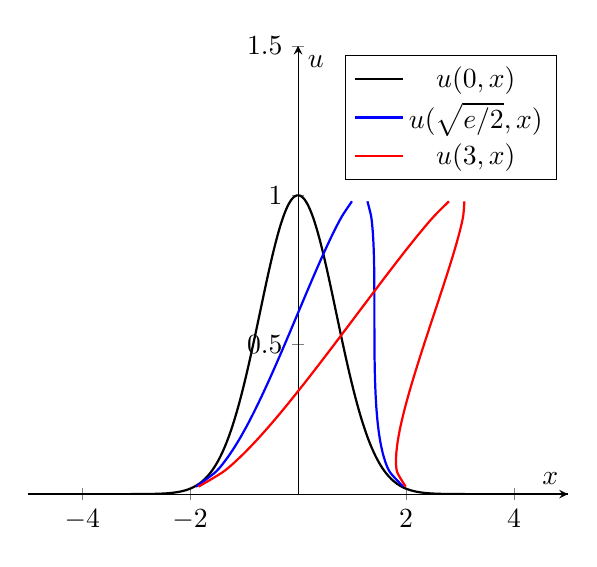
\begin{tikzpicture}
%\pgfplotsset{ %%per spostare a sinistra la legenda, copia incolla queste due righe
%every axis legend/.append style={ at={(1.05,0.95)}, anchor=north west,legend columns = 1}}
	\begin{axis} [axis lines = middle, ymin=0, ymax=1.5, xlabel={$x$}, ylabel=$u$]
            \addplot[samples=200, smooth, thick]{exp(-x^2)};
            \addlegendentry{\(u(0,x)\)}
            \addplot[variable=\t, samples=200, smooth, thick, blue]({sqrt(e/2)*t-sqrt(-ln(t))}, {t});
            \addplot[variable=\t, samples=200, smooth, thick, blue,forget plot]({sqrt(e/2)*t+sqrt(-ln(t))}, {t});
            \addlegendentry{\(u(\sqrt{e/2},x)\)}
            \addplot[variable=\t, samples=200, smooth, thick, red]({3*t-sqrt(-ln(t))}, {t});
            \addplot[variable=\t, samples=200, smooth, thick, red]({3*t+sqrt(-ln(t))}, {t});
            \addlegendentry{\(u(3,x)\)}
	\end{axis}
    \label{plot:2.1}
\end{tikzpicture}
\caption{}
\end{center}
\end{figure}

Notiamo che più $u(t,x)$ è "grande" in modulo, più la soluzione tende a muoversi verso destra velocemente. Ovviamente la soluzione in rosso (ossia per tempi maggiori di un certo valore $T$) non ha più senso, in quanto non è nemmeno una funzione. Quindi esistono dati iniziali per cui la soluzione del problema \eqref{eq:2.9} non esiste oltre un certo tempo: tale è detto tempo di catastrofe. \\
(Nel caso dell'esempio \eqref{eq:2.12} si dimostra che $T = \sqrt{\frac{e}{2}}$).
Esso, dal punto di vista del grafico della soluzione, è il primo tempo $T$ in cui $u$ ha derivata infinita in un punto $x$.
Osservando ciò che succede dalla prospettiva delle caratteristiche, si può dare un'altra interpretazione del tempo di catastrofe. Ricordando che le caratteristiche sono rette la cui pendenza dipende da $u$, abbiamo che
\begin{equation}\label{eq:2.14}
    \begin{cases}
        \frac{dx}{dt} = u\\
        x(0) = x_{0}&
    \end{cases}
    \Longrightarrow \ x = ut + x_{0} \ \Longrightarrow \ t = \frac{x-x_{0}}{u}
\end{equation}
Questa è l'equazione della retta caratteristica al variare di $x$ e $x_{0}$. Dal grafico notiamo che succede una cosa molto interessante. Rappresentiamole ad esempio congelando il tempo all'istante $t = 0$, per cui $u(0,x) = e^{-x^{2}}$.

\begin{figure}[H]
\begin{center}
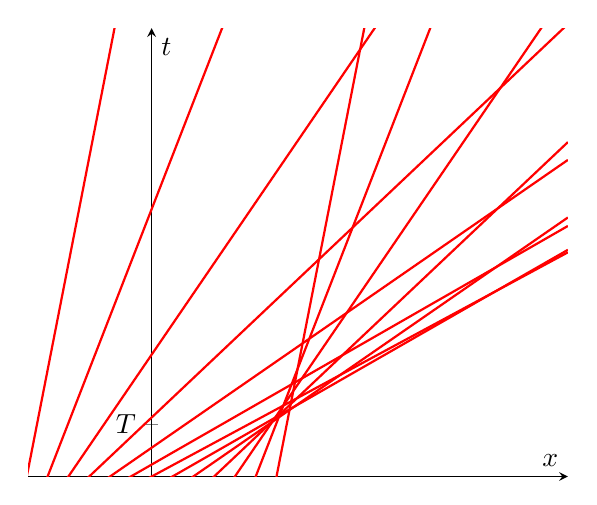
\begin{tikzpicture}
	\begin{axis} [axis lines = middle, ymin=0, ymax=10, ytick={1.165821991}, yticklabels = {$T$}, xlabel={$x$}, ylabel={$t$}, xmajorticks=false]
            \addplot[samples=200, smooth, thick, red]{9.48773583636*(x-1.5)};
            \addplot[samples=200, smooth, thick, red]{4.77073318197*(x-1.25)};
            \addplot[samples=200, smooth, thick, red]{2.71828182846*(x-1)};
            \addplot[samples=200, smooth, thick, red]{1.75505465696*(x-0.75)};
            \addplot[samples=200, smooth, thick, red]{1.28402541669*(x-0.5)};
            \addplot[samples=200, smooth, thick, red]{1.06449445892*(x-0.25)};
            \addplot[samples=200, smooth, thick, red]{x};
            \addplot[samples=200, smooth, thick, red]{1.06449445892*(x+0.25)};
            \addplot[samples=200, smooth, thick, red]{1.28402541669*(x+0.5)};
            \addplot[samples=200, smooth, thick, red]{1.75505465696*(x+0.75)};
            \addplot[samples=200, smooth, thick, red]{2.71828182846*(x+1)};
            \addplot[samples=200, smooth, thick, red]{4.77073318197*(x+1.25)};
            \addplot[samples=200, smooth, thick, red]{9.48773583636*(x+1.5)};
	\end{axis}
    \label{plot:2.2}
\end{tikzpicture}
\caption{}
\end{center}
\end{figure}

Dal grafico notiamo che non solo $T$ è il primo tempo per cui la soluzione ha una pendenza infinita in un punto $x$, $T$ è anche il primo tempo per cui due caratteristiche si incontrano. Questo è un enorme problema, sappiamo infatti che, per una soluzione classica di una PDE, vale che le curve caratteristiche, ossia le curve $(t,x(t))$ lungo le quali la soluzione è costante, non si intersecano mai. Quindi esistono problemi di Cauchy non risolvibili con soluzioni classiche, entrano allora in gioco quelle che vengono chiamate soluzioni deboli.

%%%%%%%%%%%%%%%%%%%%%%%%%%%%%%%%%%%%%%%%%%%%%%%%%%%%%%%%%%%%%%%%%%%%%%%%%%%%%%%%%%%%%%%%%%%%%%%%%%%%%%%%%%%%%%%%%%
\section{Soluzioni deboli}

In questo paragrafo, daremo la definizione di soluzione distribuzionale e di soluzione debole per un sistema di leggi di conservazione, nozioni che ci saranno di fondamentale importanza per lo studio del problema di Riemann.

\begin{definizione}
    Una funzione misurabile $u=u(t,x)$ che va da un insieme aperto $\Omega\subseteq\mathbb{R}\times\mathbb{R}$ a $\mathbb{R}^{n}$ è una soluzione distribuzionale del sistema di leggi di conservazione 
    \begin{equation}\label{eq:2.15}
        \partial_{t}u+\partial_{x}f(u)=0
    \end{equation}
    se per ogni funzione $C^{1}$ a supporto compatto $\phi\colon\Omega\longrightarrow\mathbb{R}^{n}$ si ha che 
    \begin{equation}\label{eq:2.16}
        \int\int_{\Omega}\{u\partial_{t}\phi+f(u)\partial_{x}\phi\}\,dxdt = 0.
    \end{equation}
\end{definizione}

Si osservi che nessuna ipotesi di continuità è stata fatta su $u$, richiediamo solamente che $u$ e $f(u)$ siano localmente integrabili nell'insieme $\Omega$.\\
Conseguenza immediata della definzione è il seguente lemma:
\begin{lemma}\label{lemma:2.3.1}
    Sia $\{u_{n}\}_{n\geq 1}$ una successione di soluzioni distribuzionali di \eqref{eq:2.15}.
        \begin{enumerate}[label=(\roman*)]
            \item Se
                \begin{equation}\label{eq:2.17}
                    u_{n}\rightarrow u, \ \ f(u_{n})\rightarrow f(u) \ in \ \mathbf{L}^{1}_{loc},
                \end{equation}
                allora la funzione limite $u$ è soluzione di \eqref{eq:2.15}
            \item La stessa conclusione vale se $u_{n}\rightarrow u$ in $\mathbf{L}^{1}_{loc}$ e se tutte le funzioni $u_{n}$ assumono valori in un insieme compatto.
        \end{enumerate}
\end{lemma}
\begin{proof}
    Infatti, se vale \eqref{eq:2.17}, allora per ogni $\phi\in C^{1}_{c}$ 
    \begin{equation*}
        \int\int_{\Omega}\{u\partial_{t}\phi+f(u)\partial_{x}\phi\}\,dx dt=\lim_{n\rightarrow +\infty}\int\int_{\Omega}\{u_{n}\partial_{t}\phi+f(u_{n})\partial_{x}\phi\}\,dx dt = 0,
    \end{equation*}
    mostrando così che $u$ stessa è una soluzione.\\
    Inoltre, se $u_{n}\rightarrow u$ in $\mathbf{L}^{1}_{loc}$, allora prendendo una sottosuccessione abbiamo che $u_{n}(t,x)\rightarrow u(t,x)$ quasi ovunque. Quindi anche $f(u_{n}(t,x))\rightarrow f(u(t,x))$ quasi ovunque. Le ipotesi di limitatezza su $u$ ora implicano che $f(u_{n})\rightarrow f(u)$ in $\mathbf{L}^{1}_{loc}$. L'asserto (ii) del lemma è quindi conseguenza di (i).
\end{proof}

\begin{definizione}
    Data una condizione iniziale
    \begin{equation}\label{eq:2.18}
        u(0,x) = \overline{u}(x),
    \end{equation}
    con $\overline{u}(x)\in\mathbf{L}^{1}_{loc}(\mathbb{R}, \mathbb{R}^{n})$, diciamo che una funzione $u\colon [0,T]\times\mathbb{R}\rightarrow\mathbb{R}^{n}$ è una soluzione distribuzionale del problema di Cauchy \eqref{eq:2.15}, \eqref{eq:2.18} se
    \begin{equation}\label{eq:2.19}
        \int_{0}^{T}\int_{-\infty}^{+\infty}\{u\partial_{t}\phi+f(u)\partial_{x}\phi\}\,dx dt +\int_{-\infty}^{+\infty}\overline{u}(x)\phi(0,x)\,dx = 0
    \end{equation}
    per ogni funzione $\phi\in C^{1}$ con supporto compatto contenuto nell'insieme $(-\infty, T)\times\mathbb{R}$. 
\end{definizione}

Definiamo ora un concetto più forte di soluzione, che richiede la continuità di $u$ come funzione del tempo, a valori in $\mathbf{L}^{1}_{loc}(\mathbb{R})$.

\begin{definizione}
    Una funzione $u\colon [0,T]\times\mathbb{R}\rightarrow\mathbb{R}^{n}$ è detta soluzione debole del problema di Cauchy \eqref{eq:2.15}, \eqref{eq:2.18} se $u$ è continua come funzione da $[0,T]$ a valori in $\mathbf{L}^{1}_{loc}$, la condizione iniziale \eqref{eq:2.18} vale e la restrizione di $u$ sulla striscia aperta $(0,T)\times\mathbb{R}$ è una soluzione distribuzionale di \eqref{eq:2.15}.
\end{definizione}

\begin{osservazione}
    Ogni soluzione debole è anche una soluzione in senso distribuzionale. Infatti sia $\phi\in C^{1}$ nota. Sia $\alpha\colon\mathbb{R}\rightarrow [0,2]$ una funzione liscia con supporto compatto contenuto in $(0,1)$ e tale che 
    \begin{equation*}
        \int\alpha(t)\,dt = 1.
    \end{equation*}
    Per ogni $\varepsilon >0$, definiamo le funzioni
    \begin{equation*}
        \alpha^{\varepsilon}(t) := \frac{1}{\varepsilon}\alpha(t/\varepsilon), \hspace{2cm} \beta^{\varepsilon}:=\int_{0}^{t}\alpha^{\varepsilon}(s)\,ds,
    \end{equation*}
    e definiamo $\phi^{\varepsilon}:=\phi\cdot\beta^{\varepsilon}$. Osservando che $\partial_{t}\beta^{\varepsilon}=\alpha^{\varepsilon}$ e che il supporto di $\phi^{\varepsilon}$ è contenuto in $(0,+\infty)\times\mathbb{R}$, possiamo usare la continuità della mappa $t\mapsto u(t,\cdot)$ per calcolare
    \begin{align*}
        0 &= \lim_{\varepsilon\rightarrow 0}\int_{0}^{+\infty}\int_{-\infty}^{+\infty}\{u\partial_{t}\phi^{\varepsilon}+f(u)\partial_{x}\phi^{\varepsilon}\}\,dx dt \\
        &= \lim_{\varepsilon\rightarrow 0}\int_{0}^{+\infty}\int_{-\infty}^{+\infty}\{u\partial_{t}\phi+f(u)\partial_{x}\phi\}\beta^{\varepsilon} \,dx dt + \lim_{\varepsilon\rightarrow 0}\int_{0}^{+\infty}\int_{-\infty}^{+\infty} u\phi\alpha^{\varepsilon}\, dx dt \\
        &= \int_{0}^{T}\int_{-\infty}^{+\infty}\{u\partial_{t}\phi+f(u)\partial_{x}\phi\}\, dx dt + \int_{-\infty}^{+\infty}\overline{u}(x)\phi(0,x)\, dx = 0.
    \end{align*}
    Quindi ogni soluzione debole soddisfa \eqref{eq:2.19}.
    Il viceversa è falso. Sia infatti $u=u(t,x)$ una qualunque soluzione distribuzionale non costante di \eqref{eq:2.15}, \eqref{eq:2.18}. Possiamo modificare i suoi valori per ogni tempo razionale e definire la funzione
    \begin{equation*}
    \nu(t,x):=
        \begin{cases}
            0 & \text{se} \ t>0, t\in\mathbb{Q},\\
            u(t,x) & \text{altrimenti}.
        \end{cases}
    \end{equation*}
    Siccome $\nu$ coincide con $u$ quasi ovunque nel piano $t-x$, questa nuova funzione è anch'essa una soluzione distribuzionale. Ma ovviamente $t\mapsto\nu(t,\cdot)$ è una mappa non continua a valori in $\mathbf{L}^{1}_{loc}$.
\end{osservazione}

%%%%%%%%%%%%%%%%%%%%%%%%%%%%%%%%%%%%%%%%%%%%%%%%%%%%%%%%%%%%%%%%%%%%%%%%%%%%%%%%%%%%%%%%%%%%%%%%%%%%%%%%%%%%%%%%%%
\section{Il problema di Riemann}

Sia $\Omega\subseteq\mathbb{R}^{n}$ un insieme aperto e sia $f\colon\Omega\rightarrow\mathbb{R}^{n}$ un campo vettoriale liscio. Il \textit{problema di Riemann} per un sistema di leggi di conservazione 
\begin{equation}\label{eq:2.20}
    \partial_{t}u+\partial_{x}f(u)=0
\end{equation}
consiste nel trovare una soluzione debole di \eqref{eq:2.20} con un dato iniziale costante a tratti della forma
\begin{equation}\label{eq:2.21}
    u(0,x) = 
    \begin{cases}
        u^{-} & \text{se } x<0,\\
        u^{+} & \text{se } x>0,
    \end{cases}
\end{equation}
con $u^{-}, u^{+} \in\Omega$.
Denotiamo con $A(u) = Df(u)$ la matrice Jacobiana $n\times n$ delle derivate parziali di $f$ nel punto $u$ di modo che ogni soluzione liscia di \eqref{eq:2.20} soddisfa 
\begin{equation}\label{eq:2.22}
    \partial_{t}u+A(u)\partial_{x}u=0.
\end{equation}
\begin{osservazione}
    Notiamo che se $u(t,x)$ è soluzione del problema di Riemann, allora anche la funzione $\nu(t,x) = u(at, ax)$, per ogni costante $a>0$ è soluzione dello stesso problema di Riemann, cioè le soluzioni del problema di Riemann sono invarianti per dilatazione. Infatti supponiamo $u = u(t,x)$ soluzione del problema di Riemann e consideriamo $\nu$ definita come sopra. Allora
    \begin{equation*}
        \partial_{t}\nu+\partial_{x}f(\nu) = \partial_{t}\nu+A(\nu)\partial_{x}\nu = a\partial_{t}u+A(u)a\partial_{x}u = 0.
    \end{equation*}
\end{osservazione}
Ricordiamo la definizione di sistema di leggi di conservazione strettamente iperbolico.
\begin{definizione}
    Diciamo che il sistema \eqref{eq:2.20} è strettamente iperbolico se, per ogni $u\in\Omega$, la matrice $A(u)$ ha n autovalori reali e distinti\\ $\lambda_{1}(u)< \cdots < \lambda_{n}(u)$.
\end{definizione}

Per sistemi strettamente iperbolici, si possono trovare basi di autovettori destri e sinistri $\{r_{1}(u),\ldots,r_{n}(u)\}, \{l_{1}(u),\ldots,l_{n}(u)\}$, dipendenti in maniera liscia da $u$, normalizzati in maniera tale che
\begin{equation}\label{eq:2.23}
    \|r_{i}\|\equiv 1, \hspace{1cm} l_{i}\cdot r_{j} = 
    \begin{cases}
        1 & \text{se } i = j,
        \\0 & \text{se } i\neq j, 
    \end{cases}
\end{equation}
per ogni $u\in\Omega$. Dimostriamolo in maniera rigorosa.\\
Dimostriamo anzitutto che se abbiamo una matrice iperbolica, dipendente in maniera liscia da $u$, allora anche gli autovalori dipendono in maniera liscia da $u$.
\begin{teorema}
    Sia $A\colon\Omega\rightarrow M^{n\times n}$ con $\Omega\subset\mathbb{R}^{n}$ un aperto e indicando con $M^{n\times n}$ lo spazio delle matrici $n\times n$ a coefficienti reali. Supponiamo che per ogni $u\in\Omega$, la matrice A ammetta $n$ autovalori reali e distinti
    $$\lambda_{1}(u)<\cdots <\lambda_{n}(u)$$
    (ossia A  una matrice iperbolica per ogni $u\in\Omega$) e che $A\in C^{k}(\Omega, M^{n\times n})$ con $k\geq 1$.
    Allora le funzioni $\lambda_{i}(u)\colon\Omega\rightarrow\mathbb{R}$ sono di classe $C^{k}$.
\end{teorema}
\begin{proof}
    Sia $f\colon\Omega\times\mathbb{R}\rightarrow\mathbb{R}$ definita da
    \begin{equation*}
        f(u, \lambda)=\det[A(u)-\lambda I].
    \end{equation*}
    Sia $u_{0}\in\Omega$, allora $A(u_{0})$ ha $n$ autovalori reali e distinti per cui il polinomio caratteristico può essere fattorizzato. Allora vale che
    \begin{equation*}
        f(u_{0},\lambda)=\prod_{j=1}^{n}(\lambda-\lambda_{j}(u_{0})) \hspace{1cm}\text{e}\hspace{1cm}\frac{\partial}{\partial\lambda}f(u_{0},\lambda)=\sum_{j=1}^{n}\prod_{\substack{\ell=1\\\ell\neq j}}^{n}(\lambda-\lambda_{\ell}(u_{0})).
    \end{equation*}
    Per cui ho che
    \begin{itemize}
        \item $f(u_{0},\lambda_{i}(u_{0})) = 0$,
        \item $\frac{\partial}{\partial\lambda}f(u_{0},\lambda_{i}(u_{0}))=\prod\limits_{\substack{\ell=1\\\ell\neq i}}^{n}(\lambda_{i}(u_{0})-\lambda_{l}(u_{0}))\neq 0$ \ per l'ipotesi sull'iperbolicità della matrice.
    \end{itemize}
    Allora applicando il teorema della funzione implicita, posso affermare che esiste un intorno di $\mathcal{U}(u_{0})$ e una funzione $\overline{\lambda}_{i}\colon\mathcal{U}(u_{0})\rightarrow\mathbb{R}$ di classe $C^{k}$ tale che 
    \begin{equation*}
    f(u,\overline{\lambda}_{i}(u))=0, 
    \end{equation*}
    cioè $\det[A(u)-\overline{\lambda}_{i}(u)]=0$, cioè $\overline{\lambda}_{i}(u)$ è un autovalore di $A(u)$ di classe $C^{k}$ con $\overline{\lambda}_{i}(u_{0}) = \lambda_{i}(u_{0})$ per ogni $i=1,\ldots, n$.
    Allora, poiché la matrice $A$ è iperbolica, vale che $\overline{\lambda}_{1}(u_{0})<\cdots <\overline{\lambda}_{n}(u_{0})$. Quindi per continuità esiste un intorno $\mathcal{U}(u_{0})$ tale che 
    \begin{equation*}
        \overline{\lambda}_{1}(u)<\cdots <\overline{\lambda}_{n}(u) \hspace{1cm}\text{per ogni } u\in\mathcal{U}(u_{0})
    \end{equation*}
    ma allora ho che
    \begin{equation*}
        \overline{\lambda}_{i}(u)=\lambda_{i}(u) \hspace{1cm}\text{per ogni } u\in\mathcal{U}(u_{0}), i = 1,\ldots, n
    \end{equation*}
    e quindi gli autovalori $\lambda_{i}(u)$ sono di classe $C^{k}$.
\end{proof}
\begin{teorema}
    Per ogni $u_{0}\in\Omega$ esiste un intorno $\mathcal{U}(u_{0})$ in cui gli autovettori $r_{i}(u)$ possono essere scelti  di norma unitaria, $\|r_{i}(u)\|=1$, e di classe $C^{k}$.
\end{teorema}
\begin{proof}
    Siano $r^{0}_{1},\ldots,r^{0}_{n}$ gli autovettori calcolati nel punto $u_{0}$ tali che $\|r^{0}_{i}\|=1$  per ogni $i=1,\ldots,n$ e sia $\ell^{0}_{1},\ldots,\ell^{0}_{n}$ la base duale degli autovettori sinistri, definiti da
    \begin{equation*}
        \ell^{0}_{j}\cdot r^{0}_{i} = \delta_{ij}.
    \end{equation*}
    Senza perdita di generalità, mostreremo che l'$n$-esimo autovettore può essere scelto di classe $C^{k}$ (per gli altri $n-1$ il procedimento è equivalente).
    Definiamo ora la matrice $B\colon\Omega\rightarrow M^{(n-1)\times n}$ 
    \begin{equation*}
        B(u) =
        \begin{pmatrix}\ell^{0}_{1}\cdot[A(u)-\lambda_{n}(u)I] \\ \vdots \\ \ell^{0}_{n-1}\cdot[A(u)-\lambda_{n}(u)I]\end{pmatrix}\\
    \end{equation*}
    di classe $C^{k}$. Allora, calcolando la matrice $B(u)$ nel punto $u_{0}$ e utilizzando il fatto che $\ell^{0}_{i}$ è un autovettore sinistro per ogni $i=1,\ldots,n-1$, otteniamo che
    \begin{equation*}
        B(u_{0}) =
        \begin{pmatrix}\ell^{0}_{1}\cdot[A(u_{0})-\lambda_{n}(u_{0})I] \\ \vdots \\ \ell^{0}_{n-1}\cdot[A(u_{0})-\lambda_{n}(u_{0})I]\end{pmatrix}\\ = 
        \begin{pmatrix}\ell^{0}_{1}\cdot[\lambda_{1}(u_{0})-\lambda_{n}(u_{0})] \\ \vdots \\ \ell^{0}_{n-1}\cdot[\lambda_{n-1}(u_{0})-\lambda_{n}(u_{0})]\end{pmatrix}\\.
    \end{equation*}
    Poiché $\lambda_{i}(u_{0})-\lambda_{n}(u_{0})\neq 0$ per ogni $i = 1,\ldots,n-1$, il rango di $B(u_{0})$ è $n-1$, cioè le righe di $B(u_{0})$ sono linearmente indipendenti. Quindi per continuità esiste un intorno di $u_{0}$, $\overline{\mathcal{U}}(u_{0})$ in cui $B(u)$ ha le righe linearmente indipendenti.\\
    Sia ora $F\colon\Omega\times\mathbb{R}^{n}\rightarrow\mathbb{R}^{n}$ definita da
    \begin{equation*}
        F(u,y) = \begin{pmatrix}B(u)y \\ \ell_{n}^{0}\cdot y-1\end{pmatrix}
        = \begin{pmatrix}\ell^{0}_{1}\cdot[A(u)-\lambda_{n}(u)I]y \\ \vdots \\ \ell^{0}_{n-1}\cdot[A(u)-\lambda_{n}(u)I]y\\ \ell_{n}^{0}\cdot y-1\end{pmatrix}\\
    \end{equation*}
    e osserviamo che 
    \begin{itemize}
        \item $F(u_{0},r^{0}_{n})=
        \begin{pmatrix}\ell^{0}_{1}\cdot[A(u_{0})-\lambda_{n}(u_{0})I]r^{0}_{n} \\ \vdots \\ \ell^{0}_{n-1}\cdot[A(u_{0})-\lambda_{n}(u_{0})I]r^{0}_{n}\\ \ell_{n}^{0}\cdot r^{0}_{n}-1\end{pmatrix} = \left(\begin{array}{c}0\\ \vdots\\0\end{array}\right)\\$
        \item$D_{2}F(u_{0},r_{n}^{0})=
        \begin{pmatrix}\ell^{0}_{1}\cdot[\lambda_{1}(u_{0})-\lambda_{n}(u_{0})] \\ \vdots \\ \ell^{0}_{n-1}\cdot[\lambda_{n-1}(u_{0})-\lambda_{n}(u_{0})]\\ \ell_{n}^{0}\end{pmatrix}\\
        \Rightarrow\det D_{2}F(u_{0},r^{0}_{n})\neq 0.$
    \end{itemize}
    Allora per il teorema della funzione implicita esiste un intorno $\mathcal{U}(u_{0})\subset\overline{\mathcal{U}}(u_{0})$ e una funzione $\widetilde{r}_{n}\colon\mathcal{U}(u_{0})\rightarrow\mathbb{R}^{n}$ di classe $C^{k}$ tale che
    \begin{equation*}
        F(u,\widetilde{r}_{n}(u)) = 0,
    \end{equation*}
    cioè 
    \begin{equation*}
        \begin{cases}
            \ell^{0}_{i}\cdot[A(u)-\lambda_{n}(u)I]\widetilde{r}_{n}(u)=0 & \text{per } i = 1,\ldots,n-1,\nonumber\\
            \ell_{n}^{0}\cdot\widetilde{r}_{n}(u)-1=0 .&
        \end{cases}
    \end{equation*}
    Dall'ultima relazione ricavo che $\widetilde{r}_{n}(u)\neq 0$.
    Ora, poiché $\lambda_{n}(u)$ è un autovalore, ho che $\det[A(u)-\lambda_{n}(u)I] = 0$ e quindi le righe 
    $$\begin{array}{cc}
      \ell^{0}_{1}\cdot[A(u)-\lambda_{n}(u_{0})I]\\
      \vdots \\
      \ell^{0}_{n}\cdot[A(u)-\lambda_{n}(u_{0})I]
    \end{array}$$
    sono linearmente dipendenti, sapendo che le prime $n-1$ righe sono linearmente indipendenti. Questo mi dice che la riga $n$-esima è combinazione lineare delle $n-1$ precedenti, cioè
    \begin{equation*}
        \ell^{0}_{n}\cdot[A(u)-\lambda_{n}(u)I] = \sum_{i=1}^{n-1}\alpha_{i}(u)\ell_{i}^{0}\cdot[A(u)-\lambda_{n}(u)I]
    \end{equation*}
    per certi coefficienti $\alpha_{i}(u)$. Per cui
    \begin{equation*}
        \ell^{0}_{n}\cdot[A(u)-\lambda_{n}(u)I]\widetilde{r}_{n}(u) = \sum_{i=1}^{n-1}\alpha_{i}(u)\ell_{i}^{0}\cdot[A(u)-\lambda_{n}(u)I]\widetilde{r}_{n}(u) = 0.
    \end{equation*}
    Quindi $\ell^{0}_{i}\cdot[A(u)-\lambda_{n}(u)I]\widetilde{r}_{n}(u) =0$ per ogni $i=1,\ldots,n$. Questo implica che $[A(u)-\lambda_{n}(u)I]\widetilde{r}_{n}(u)=0$, cioè $\widetilde{r}_{n}(u)$ è autovettore di classe $C^{k}$ in $\mathcal{U}(u_{0})$ con autovalore $\lambda_{n}(u)$ ed essendo $\widetilde{r}_{n}(u)\neq 0$, possiamo definire 
    \begin{equation*}
        r_{n}(u) = \frac{\widetilde{r}_{n}(u)}{\|\widetilde{r}_{n}(u)\|} 
    \end{equation*}
    per ottenere l'autovettore di classe $C^{k}$ con norma unitaria.
\end{proof}
Abbiamo quindi dimostrato che esistono basi di autovettori destri e sinistri come in \eqref{eq:2.23} che dipendono in maniera liscia da $u$.\\
Nel seguito, indicheremo la derivata direzionale di una funzione $\phi=\phi(u)$, lungo la direzione del vettore $r_{i}(u)$, come 
\begin{equation*}
    r_{i}\bullet\phi(u) := D\phi(u)\cdot r_{i}=\lim_{\varepsilon\rightarrow 0}\frac{\phi(u+\varepsilon r_{i}(u))-\phi(u)}{\varepsilon}.
\end{equation*}

\begin{definizione}
    Per $i\in\{1, \ldots, n\}$, diciamo che l'i-esimo campo caratteristico è genuinamente non lineare se
    \begin{equation*}
        r_{i}\bullet\lambda_{i}(u)\neq 0 \text{ per ogni } u\in\Omega.
    \end{equation*}
    Se invece
    \begin{equation*}
        r_{i}\bullet\lambda_{i}(u)= 0 \text{ per ogni } u\in\Omega,
    \end{equation*}
    diciamo che l'i-esimo campo caratteristico è linearmente degenere.
\end{definizione}

Ricordiamo brevemente la definizione di curva integrale:
\begin{definizione}
    Sia $F$ un campo vettoriale, cioè una funzione vettoriale con coordinate cartesiane $(F_{1}, F_{2}, \ldots , F_{n})$ e sia $x(t)$ una curva parametrica avente coordinate $(x_{1}(t), x_{2}(t), \ldots, x_{n}(t))$. Allora $x(t)$ è detta essere curva integrale del campo vettoriale $F$ se è una soluzione del seguente sistema di equazioni differenziali ordinarie
    \begin{align}\label{eq:2.24}
        \frac{dx_{1}}{dt}&=F_{1}(x_{1},\ldots,x_{n}),\nonumber \\
        &\vdots\nonumber \\
        \frac{dx_{n}}{dt}&=F_{n}(x_{1},\ldots,x_{n}).
    \end{align}
    La definizione afferma che il vettore tangente alla curva in ogni punto $x(t)$ lungo la curva è precisamente il vettore F(x(t)).
\end{definizione}
Osserviamo che, per la continuità delle derivate prime, nel caso di campo caratteristico genuinamente non lineare il valore di $\lambda_{i}$ è strettamente monotono (crescente o decrescente) lungo ogni curva integrale del campo vettoriale $r_{i}$. Cambiando il segno di $r_{i}$, possiamo supporre quindi che 
\begin{equation}\label{eq:2.25}
    r_{i}\bullet\lambda_{i}(u)>0 \text{ per ogni } u\in\Omega.
\end{equation}
D'altra parte, nel caso di campo caratteristico linearmente degenere l'autovalore $\lambda_{i}=\lambda_{i}(u)$ è costante lungo ogni curva integrale di $r_{i}$.
In questo capitolo costruiremo soluzioni deboli del problema di Riemann \eqref{eq:2.20}-\eqref{eq:2.21}, per $u^{-}, u^{+}$  sufficientemente vicini, sotto la seguente ipotesi:
\begin{description}
    \item {$(\clubsuit)$} Il sistema \eqref{eq:2.20} è strettamente iperbolico con coefficienti regolari, definiti in un insieme aperto $\Omega\subseteq\mathbb{R}^{n}$. Per ogni $i\in\{1,\ldots,n\}$, l'i-esimo campo caratteristico è o genuinamente lineare oppure linearmente degenere.
\end{description}
La soluzione si dimostrerà essere autosimilare, ossia avente la forma \\$u(x,t)=\psi(x/t)$, con $\psi\colon\mathbb{R}\rightarrow\mathbb{R}^{n}$ possibilmente discontinua.

%%%%%%%%%%%%%%%%%%%%%%%%%%%%%%%%%%%%%%%%%%%%%%%%%%%%%%%%%%%%%%%%%%%%%%%%%%%%%%%%%%%%%%%%%%%%%%%%%%%%%%%%%%%%%%%%%%
\section{Curve di rarefazione}

Nel seguito, con $\sigma\mapsto R_{i}(\sigma)(u_{0})$ intendiamo la curva integrale parametrizzata dell'autovettore $r_{i}$ attraverso il punto $u_{0}$. Più precisamente, $R_{i}(\sigma)(u_{0})$ è la soluzione del problema di Cauchy
\begin{equation}\label{eq:2.26}
    \frac{du}{d\sigma}=r_{i}(u(\sigma)), \hspace{2cm} u(0)=u_{0}.
\end{equation}
dove ricordiamo che $r_{i}$ è l'$i$-esimo autovettore destro della matrice $Df$.
La curva $R_{i}$ è chiamata la \textit{i-esima curva di rarefazione} passante per $u_{0}$. Avendo definito la curva $R_{i}$ in termini della soluzione di una equazione differenziale ordinaria (ODE) con coefficienti lisci, abbiamo le seguenti identità
\begin{align}
    \frac{d}{d\sigma}R_{i}(\sigma)(u_{0}) &= r_{i}(R_{i}(\sigma)(u_{0})), \label{eq:2.27}\\
    R_{i}(\sigma ')(R_{i}(\sigma)(u_{0})) &= R_{i}(\sigma+\sigma ')(u_{0}), \label{eq:2.28}
\end{align}
per ogni $u_{0}, \sigma, \sigma '$.\\
Ora siano $u^{-}, u^{+}$ assegnati. Assumiamo che esista un campo caratteristico genuinamente non lineare di autovettori $r_{i}$ soddisfacente \eqref{eq:2.25}, e per qualche $\overline{\sigma}\geq 0$
\begin{equation}\label{eq:2.29}
    u^{+}=R_{i}(\overline{\sigma})(u^{-}).
\end{equation}
In questo caso la soluzione del problema di Riemann si può costruire come segue. Osserviamo che, per la genuina non linearità, la funzione
\begin{equation}\label{eq:2.30}
    \sigma\mapsto\lambda_{i}(R_{i}(\sigma)(u^{-}))
\end{equation}
è strettamente crescente (quindi invertibile) e mappa l'intervallo $\left[0,\hspace{0.075cm} \overline{\sigma}\right]$ in $\left[\lambda_{i}(u^{-}),\hspace{0.075cm}\lambda_{i}(u^{+})\right]$. Per $t>0$, possiamo definire la seguente funzione lipschitziana definita a tratti
\begin{equation}\label{eq:2.31}
    u(t,x) = 
    \begin{cases}
        u^{-} & \text{se} \ x/t<\lambda_{i}(u^{-}),\\
        u^{+} & \text{se} \ x/t>\lambda_{i}(u^{+}),\\
        R_{i}(\sigma)(u^{-}) & \text{se} \ x/t\in\left[\lambda_{i}(u^{-}),\hspace{0.075cm}\lambda_{i}(u^{+})\right],\ x/t=\lambda_{i}(R_{i}(\sigma)(u^{-})).
    \end{cases}
\end{equation}
Questa è una soluzione debole di \eqref{eq:2.20}-\eqref{eq:2.21}. Infatti, $u(t,\cdot)\rightarrow u(0,\cdot)$ in $\mathbf{L}^{1}_{loc}$ per $t\rightarrow 0^{+}$. Inoltre, l'equazione \eqref{eq:2.22} è soddisfatta nelle regioni dove $x/t < \lambda_{i}(u^{-})$ oppure $x/t>\lambda_{i}(u^{+})$. Sia ora $x/t\in [\lambda_{i}(u^{-}),\lambda_{i}(u^{+})]$ e consideriamo la $i$-esima curva di rarefazione $u(t,x)=R_{i}(\sigma)(u^{-})$ ove $\sigma = \Lambda_{i}^{-1}(x/t)$ e abbiamo denotato $\Lambda_{i}(\sigma) = \lambda_{i}(R_{i}(\sigma)(u^{-}))$, che sappiamo essere invertibile perché strettamente crescente. Allora (indicando con $\frac{d}{d\sigma} R_{i}=R_{i}' $)
\begin{align*}
    \partial_{t}u+\partial_{x}f(u) &= \partial_{t}u+Df(u)\partial_{x}u\\
    &= R_{i}'(\sigma)(u^{-})\partial_{t}\sigma + Df(u)R_{i}'(\sigma)(u^{-})\partial_{x}\sigma\\
    &=R_{i}'(\sigma)(u_{0})\partial_{t}\sigma+\lambda_{i}(u)R_{i}'(\sigma)(u_{0})\partial_{x}\sigma\\
    &=R_{i}'(\sigma)(u_{0})\left[\partial_{t}\sigma + \lambda_{i}(R_{i}(\sigma)(u^{-}))\partial_{x}\sigma\right]\\
    &=R_{i}'(\sigma)(u_{0})\left[\partial_{t}\sigma + \frac{x}{t}\partial_{x}\sigma\right] = 0
\end{align*}
perché $\sigma$ dipende unicamente da $x/t$.
Allora \eqref{eq:2.22} vale anche nella regione $\lambda_{i}(u^{-})<x/t<\lambda_{i}(u^{+})$.\\
Una soluzione del problema di Riemann avente la forma \eqref{eq:2.31} è detta \textit{onda di rarefazione}.
\begin{osservazione}
    Sappiamo che, per definizione di curva di rarefazione come curva integrale $R_{i}'(\sigma)(u_{0})=r_{i}(R_{i}(\sigma)(u_{0})$. Calcoliamo la derivata seconda della $i$-esima curva di rarefazione:
    \begin{align}
        \frac{d^{2}}{d\sigma^{2}}R_{i}(\sigma)(u_{0}) &= \frac{d}{d\sigma}\left(\frac{d}{d\sigma}R_{i}(\sigma)(u_{0})\right)\nonumber\\
        &=\frac{d}{d\sigma}r_{i}(R_{i}(\sigma)(u_{0}))\nonumber\\
        &= Dr_{i}(R_{i}(\sigma)(u_{0}))\cdot \frac{d}{d\sigma}R_{i}(\sigma)(u_{0})\nonumber\\
        &= Dr_{i}(R_{i}(\sigma)(u_{0}))\cdot r_{i}(R_{i}(\sigma)(u_{0})\nonumber\\
        &= r_{i}\bullet r_{i}(R_{i}(\sigma)(u_{0})).
    \end{align}
\end{osservazione}
\begin{esempio}
    Consideriamo l'equazione di Burgers inviscida
    \begin{equation}\label{eq:2.33}
        \partial_{t}u+\partial_{x}\left(\frac{u^{2}}{2}\right)=0,
    \end{equation}
    con condizione iniziale
    \begin{equation}\label{eq:2.34}
        u(0,x)=
        \begin{cases}
            1\text{ se }x>0,\\
            0\text{ se }x<0.
        \end{cases}
    \end{equation}
    Notiamo che le caratteristiche di tale problema sono
\begin{figure}[H]
\begin{center}
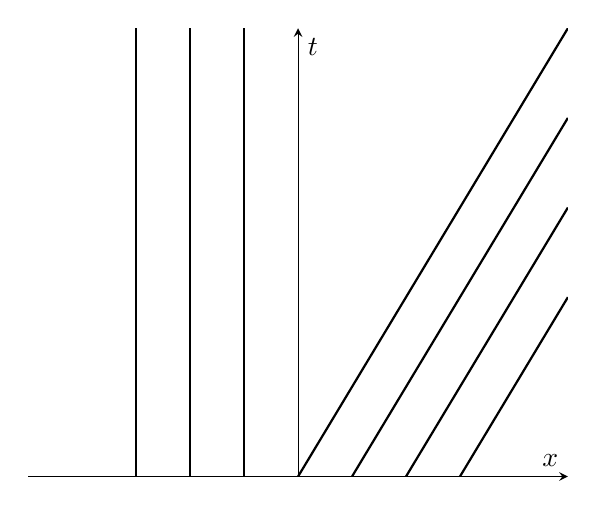
\begin{tikzpicture}
	\begin{axis} [axis lines = middle, ymin=0, ymax=5, xmin=-5, xmax=5, xlabel={$x$}, ylabel={$t$}, xmajorticks=false, ymajorticks=false]
            \addplot[samples=200, smooth, thick]coordinates{(-3,0)(-3,5)};
            \addplot[samples=200, smooth, thick]coordinates{(-2,0)(-2,5)};
            \addplot[samples=200, smooth, thick]coordinates{(-1,0)(-1,5)};
            \addplot[samples=200, smooth, thick]{x};
            \addplot[samples=200, smooth, thick]{x-1};
            \addplot[samples=200, smooth, thick]{x-2};
            \addplot[samples=200, smooth, thick]{x-3};
	\end{axis}
    \label{plot:2.3}
\end{tikzpicture}
\caption{}
\end{center}
\end{figure}
Ci chiediamo in che modo poter "riempire" la regione vuota. Una soluzione potrebbe essere usare delle curve della forma $x = ct$ con $c$ costante che varia all'interno dell'intervallo $[0,1]$, ottenendo quindi
\begin{figure}[H]
\begin{center}
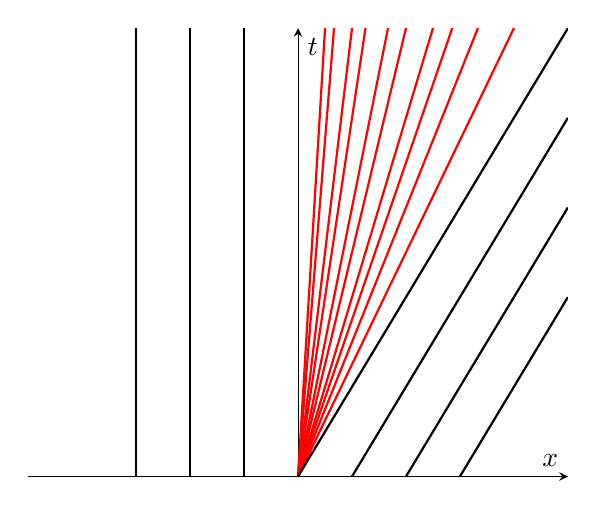
\begin{tikzpicture}
	\begin{axis} [axis lines = middle, ymin=0, ymax=5, xmin=-5, xmax=5, xlabel={$x$}, ylabel={$t$}, xmajorticks=false, ymajorticks=false]
            \addplot[samples=200, smooth, thick]coordinates{(-3,0)(-3,5)};
            \addplot[samples=200, smooth, thick]coordinates{(-2,0)(-2,5)};
            \addplot[samples=200, smooth, thick]coordinates{(-1,0)(-1,5)};
            \addplot[samples=200, smooth, thick, red]{10*x};
            \addplot[samples=200, smooth, thick, red]{7.5*x};
            \addplot[samples=200, smooth, thick, red]{5*x};
            \addplot[samples=200, smooth, thick, red]{4*x};
            \addplot[samples=200, smooth, thick, red]{3*x};
            \addplot[samples=200, smooth, thick, red]{2.5*x};
            \addplot[samples=200, smooth, thick, red]{2*x};
            \addplot[samples=200, smooth, thick, red]{1.75*x};
            \addplot[samples=200, smooth, thick, red]{1.5*x};
            \addplot[samples=200, smooth, thick, red]{1.25*x};
            \addplot[samples=200, smooth, thick]{x};
            \addplot[samples=200, smooth, thick]{x-1};
            \addplot[samples=200, smooth, thick]{x-2};
            \addplot[samples=200, smooth, thick]{x-3};
	\end{axis}
    \label{plot:2.4}
\end{tikzpicture}
\caption{}
\end{center}
\end{figure}
Si noti che tali soluzioni sono costruite in modo tale che vanno con continuità dalle rette con pendenza verticale a quelle con pendenza pari a 1. Allora la soluzione è data da
\begin{equation}\label{eq:2.35}
    u(t,x)=
    \begin{cases}
        0\text{ se }x<0,\\
        x/t\text{ se }0<x<t,\\
        1\text{ se }x>t.
    \end{cases}
\end{equation}
\end{esempio}

%%%%%%%%%%%%%%%%%%%%%%%%%%%%%%%%%%%%%%%%%%%%%%%%%%%%%%%%%%%%%%%%%%%%%%%%%%%%%%%%%%%%%%%%%%%%%%%%%%%%%%%%%%%%%%%%%%
\section{Condizioni di Rankine-Hugoniot}
In questa sezione considereremo una funzione $u$ lipschitziana a tratti, con discontinuità di salto lungo un numero finito di curve nel piano $t-x$. Il nostro obiettivo è di derivare delle condizioni che garantiscano che $u$ sia una soluzione di \eqref{eq:2.20}. Per risolvere il nostro problema, ci viene in soccorso il seguente teorema
\begin{teorema}
    Sia $x\colon [0,+\infty)\rightarrow\mathbb{R}$ una funzione lipschitziana, 
    \begin{equation*}
        \Omega^{-}=\{(t,x)\in\mathbb{R}^{2}|t\geq 0 \ \wedge \ x\leq x(t)\}, \hspace{1cm} \Omega^{+}=\{(t,x)\in\mathbb{R}^{2}|t\geq 0 \ \wedge \ x\geq x(t)\}
    \end{equation*}
    e siano $g^{-}, f^{-}\in C^{1}(\Omega^{-},\mathbb{R})$, $g^{+}, f^{+}\in C^{1}(\Omega^{+},\mathbb{R})$ tali che
    \begin{equation*}
        \partial_{t}g^{\pm} + \partial_{x}f^{\pm}=0 \text{ in } \Omega^{\pm}.
    \end{equation*}
    Definiamo
    \begin{equation*}
        f(t,x) =
        \begin{cases}
            f^{-}(t,x) & \text{se} \ (t,x)\in\Omega^{-}, \\
            f^{+}(t,x) & \text{se} \ (t,x)\in\Omega^{+}
        \end{cases}
        ,\hspace{1cm} g(t,x) =
        \begin{cases}
            g^{-}(t,x) & \text{se} \ (t,x)\in\Omega^{-}, \\
            g^{+}(t,x) & \text{se} \ (t,x)\in\Omega^{+}.
        \end{cases}
    \end{equation*}
    Allora $\partial_{t}g+\partial_{x}f=0$ in senso debole se e solo se vale la seguente condizione:
    \begin{equation}\label{eq:2.36}
        \dot{x}(t)\Delta g(t,x(t)) = \Delta f(t,x(t))
    \end{equation}
     con 
     \begin{equation*}
         \Delta g(t,x(t))=g^{+}(t,x(t))-g^{-}(t,x(t)) \text{ e } \Delta f(t,x(t))=f^{+}(t,x(t))-f^{-}(t,x(t))
     \end{equation*}
     per quasi ogni $t\geq 0$.
\end{teorema}
\begin{proof}
    Sia $\phi\in C^{1}_{c}((0,+\infty)\times\mathbb{R},\mathbb{R})$.\\
    Allora, affinché $f$ e $g$ siano soluzioni deboli di \eqref{eq:2.20} se
    \begin{align*}
        0 = \int_{\Omega^{+}\cup\Omega^{-}}g\partial_{t}\phi+f\partial_{x}\phi\,dtdx = \int_{\Omega^{-}}g^{-}\partial_{t}\phi&+f^{-}\partial_{x}\phi\,dtdx \\&+ \int_{\Omega^{+}}g^{+}\partial_{t}\phi+f^{+}\partial_{x}\phi\,dtdx
    \end{align*}
    Ora, osserviamo che
    \begin{align*}
        &\int_{\Omega^{-}}g^{-}\partial_{t}\phi+f^{-}\partial_{x}\phi\,dtdx =\\
        &=\int_{0}^{+\infty}\int_{-\infty}^{x(t)}[g^{-}(t,x)\partial_{t}\phi(t,x)+f^{-}(t,x)\partial_{x}\phi(t,x)]\,dtdx \\
        &= \int_{0}^{+\infty}\int_{-\infty}^{x(t)}\partial_{t}[g^{-}(t,x)\phi(t,x)]-\partial_{t}g^{-}(t,x)\phi(t,x)\\
        &\hphantom{=}\hspace{5cm}+\partial_{x}[f^{-}(t,x)\phi(t,x)]-\partial_{x}f^{-}(t,x)\phi(t,x)\,dxdt \\
        &\text{dato che $\partial_{t}g^{-}+\partial_{x}f^{-}=0$ per ipotesi, il secondo e il quarto termine si }\\
        &\text{elidono. Continuando con il nostro calcolo, si ha che}\\
        &= \int_{0}^{+\infty}\int_{-\infty}^{x(t)}\partial_{t}[g^{-}(t,x)\phi(t,x)]+\partial_{x}[f^{-}(t,x)\phi(t,x)]\,dxdt \\
        &= \int_{0}^{+\infty}\int_{-\infty}^{x(t)}\partial_{t}[g^{-}(t,x)\phi(t,x)]\,dxdt + \int_{0}^{+\infty}\int_{-\infty}^{x(t)}\partial_{x}[f^{-}(t,x)\phi(t,x)]\,dxdt \\
        &= \int_{0}^{+\infty}\int_{-\infty}^{x(t)}\partial_{t}[g^{-}(t,x)\phi(t,x)]\,dxdt + \int_{0}^{+\infty}f^{-}(t,x(t))\phi(t,x(t))\,dt\\
        &\text{Eseguendo il cambio di variabile $x = x(t) + y$}\\
        &=\int_{0}^{+\infty}\int_{-\infty}^{0}D_{1}[g^{-}(t,x(t)+y)]\phi(t,x(t)+y)]\,dydt \\ &\hspace{1cm}+\int_{0}^{+\infty}f^{-}(t,x(t))\phi(t,x(t))\,dt\\
        &= \int_{0}^{+\infty}\int_{-\infty}^{0}\partial_{t}[g^{-}(t,x(t)+y)\phi(t,x(t)+y)] \\ & \hspace{1cm} -\partial_{y}[g^{-}(t,x(t)+y)\phi(t,x(t)+y)]\dot{x}(t)\,dydt  + \int_{0}^{+\infty}f^{-}(t,x(t))\phi(t,x(t))\,dt\\
        &= \int_{-\infty}^{0}\left(\int_{0}^{+\infty}\partial_{t}[g^{-}(t,x(t)+y)\phi(t,x(t)+y)]\,dt\right)\,dy 
        \\ & \hspace{1cm} -\int_{0}^{+\infty}g^{-}(t,x(t))\phi(t,x(t))\dot{x}(t)\,dt +\int_{0}^{+\infty}f^{-}(t,x(t))\phi(t,x(t))\,dt\\
        &\text{Ora, poiché $\phi\in C^{1}_{c}((0, +\infty)\times\mathbb{R}, \mathbb{R})$, l'integrale tra parentesi è nullo,}\\ &\text{e quindi tutto il primo termine vale zero.}\\
        &=\int_{0}^{+\infty}[f^{-}(t,x(t))-g^{-}(t,x(t))\dot{x}(t)]\phi(t,x(t))\,dt.
    \end{align*}

    \hspace{-0.5cm}Eseguendo lo stesso conto in $\Omega^{+}$, otteniamo infine che 
    \begin{equation*}
        \int_{\Omega^{-}\cup\Omega^{+}}[\partial_{t}\phi+f\partial_{x}\phi]\,dtdx = \int_{0}^{+\infty}[\Delta g(t,x(t))\dot{x}(t)-\Delta f(t,x(t))]\phi(t,x(t))\,dt.
    \end{equation*}
    Per l'arbitrarietà di $\phi$, segue la tesi.
\end{proof}

L'equazione vettoriale \eqref{eq:2.36} sono dette \textit{condizioni di Rankine-Hugoniot}.
Considerando il caso particolare in cui
\begin{equation}\label{eq:2.37}
    U(t,x) = 
    \begin{cases}
        u^{+} & \text{se} \ x>\lambda t, \\
        u^{-} & \text{se} \ x<\lambda t,
    \end{cases}
\end{equation}
per qualche $u^{-}, u^{+}\in\mathbb{R}^{n}, \lambda\in\mathbb{R}$, e in cui $g(t,x)=U(t,x)$ e $f(t,x)=f(U(t,x))$ allora dal teorema precedente si ricava il seguente lemma
\begin{lemma}\label{lemma:2.6.1}
    La funzione U definita in \eqref{eq:2.37} è una soluzione di \eqref{eq:2.20} se e solo se
    \begin{equation}\label{eq:2.38}
        \lambda(u^{+}-u^{-})=f(u^{+})-f(u^{-}).
    \end{equation}
\end{lemma}

Queste formano un sistema di $n$ equazioni scalari che mettono in relazione lo stato destro e sinistro $u^{+}, u^{-}\in\mathbb{R}^{n}$ e la velocità della discontinuità $\lambda$.

\begin{osservazione}
    Indicando con $A(u) = Df(u)$ la matrice Jacobiana $n\times n$ di $f$ in $u$. Assumendo che il segmento congiungente i due stati $u, \nu$ è interamente contenuto nel dominio di $f$, definiamo la matrice media
    \begin{equation}\label{eq:2.39}
        A(u,\nu) :=\int_{0}^{1}A(\theta u+(1-\theta)\nu)\,d\theta
    \end{equation}
    e chiamiamo $\lambda_{i}(u,\nu), i = 1,\ldots,n$, i suoi autovalori. Allora possiamo scrivere \eqref{eq:2.38} nella forma equivalente
    \begin{align}\label{eq:2.40}
        \lambda\left(u^{+}-u^{-}\right) &= f(u^{+})-f(u^{-}) = \int_{0}^{1}Df(\theta u^{+}+(1-\theta)u^{-})\cdot (u^{+}-u^{-})\,d\theta \nonumber\\
        &=A(u^{+},u^{-})\cdot (u^{+}-u^{-}).
    \end{align}
    In altre parole, le condizioni di Rankine-Hugoniot valgono se e solo se il salto $u^{+}-u^{-}$ è un autovettore della matrice media $A(u^{+},u^{-})$ e la velocità $\lambda$ concide con il corrispondente autovalore.
\end{osservazione}

\begin{osservazione}
    Nel caso in cui $f$ sia lipschitziana, denotando con $Lip(f)$ la costante di Lipschitz di $f$, otteniamo dalla \eqref{eq:2.38} un limite superiore per la velocità del salto:
    \begin{equation}\label{eq:2.41}
        |\lambda|\leq Lip(f).
    \end{equation}
\end{osservazione}

\begin{osservazione}\label{osservazione 2.6.3}
    Se $u^{+}\neq u^{-}$, la funzione
    \begin{equation}\label{eq:2.42}
        U(t,x) := 
        \begin{cases}
            u^{+} & \text{se} \ t>0, \\
            u^{-} & \text{se} \ t<0
        \end{cases}
    \end{equation}
    non può essere una soluzione di \eqref{eq:2.20}. Infatti, applicare il teorema della divergenza in questo caso porta a
    \begin{equation}\label{eq:2.43}
        0 = \int\int\{U\partial_{t}\phi+f(U)\partial_{x}\phi\}\,dxdt = -\int [u^{+}-u^{-}]\phi(0,x)\,dx.
    \end{equation}
    Se \eqref{eq:2.43} valesse per ogni $\phi\in C^{1}_{c}$, allora avrei che $u^{+}=u^{-}$ che però contraddice l'ipotesi.
\end{osservazione}

\begin{esempio}
    Per l'equazione di Burger inviscida
    \begin{equation}\label{eq:2.44}
        \partial_{t}u+\partial_{x}\left(\frac{u^{2}}{2}\right)=0,
    \end{equation}
    lungo ogni curva di shock $x=\gamma(t)$ la condizioni di Rankine-Hugoniot si riducono a
    \begin{equation}\label{eq:2.45}
        \dot{\gamma}(t)=\frac{[(u^{+})^{2}/2]-[(u^{-})^{2}/2]}{u^{+}-u^{-}}=\frac{u^{+}+u^{-}}{2}=\lambda.
    \end{equation}
    Una soluzione debole di \eqref{eq:2.44} con condizione iniziale
    \begin{equation}\label{eq:2.46}
        u(0,x) = 
        \begin{cases}
            0 & \text{se} \ x>0, \\
            1 & \text{se} \ x<0
        \end{cases}
    \end{equation}
    è data dalla funzione
    \begin{equation}\label{eq:2.47}
        u(t,x) = 
        \begin{cases}
            0 & \text{se} \ x > t/2, \\
            1 & \text{se} \ x < t/2.
        \end{cases}
    \end{equation}
\end{esempio}

%%%%%%%%%%%%%%%%%%%%%%%%%%%%%%%%%%%%%%%%%%%%%%%%%%%%%%%%%%%%%%%%%%%%%%%%%%%%%%%%%%%%%%%%%%%%%%%%%%%%%%%%%%%%%%%%%%

\section{Curve di Shock}

L'obiettivo di questo paragrafo è risolvere il seguente problema: dato $u_{0}\in\Omega$, vogliamo trovare $u, \lambda$ tali per cui si ha che
\begin{equation}\label{eq:2.48}
    f(u)-f(u_{0}) = \lambda(u-u_{0})
\end{equation}
con $f$ di classe $C^{k+1}$.
Dato un parametro reale $\sigma$, per il seguito, conviene scrivere $u = u_{0}+\sigma r$, con $r\in\mathbb{R}^{n}$ vettore, cioé
\begin{equation*}
    r = \frac{1}{\sigma}(u-u_{0}) \text{ se } \sigma\neq 0.
\end{equation*}
Quindi otteniamo che
\begin{align}\label{eq:2.49}
    f(u)-f(u_{0})&=\int_{0}^{1}Df(u_{0}+s(u-u_{0}))\,ds\cdot (u-u_{0})\nonumber\\
                 &=\sigma\int_{0}^{1}Df(u_{0}+s\sigma r)\,ds\cdot r
\end{align}
Mettendo insieme \eqref{eq:2.48} con \eqref{eq:2.49} otteniamo che
\begin{equation*}
    \sigma\int_{0}^{1}Df(u_{0}+s\sigma r)\,ds\cdot r = \lambda(u-u_{0})=\lambda\sigma r
\end{equation*}
e quindi 
\begin{equation}\label{eq:2.50}
    \int_{0}^{1}Df(u_{0}+s\sigma r)\,ds\cdot r = \lambda r.
\end{equation}
Definiamo ora 
\begin{equation}\label{eq:2.51}
    A(u_{0},v)=\int_{0}^{1}Df(u_{0}+sv)\,ds
\end{equation}
di classe $C^{k}$. Allora ho che $A(u_{0},0) = Df(u_{0}) = A(u_{0})$. Allora la \eqref{eq:2.50} equivale a chiedere che $[A(u_{0},\sigma r)-\lambda I]r = 0$, cioè $r$ deve essere autovettore di $A(u_{0},\sigma r)$ con autovalore $\lambda$.
Per cui dati $K\subset \Omega$ compatto, $\mathcal{U}(0)\subset\mathbb{R}$ un intorno di 0 e $W\subset\mathbb{R}^{n}$ aperto limitato contente la palla unitaria, introduciamo la funzione $F\colon K\times\mathcal{U}(0)\times W\times\mathbb{R}\rightarrow\mathbb{R}^{n+1}$ definita da
\begin{equation}\label{eq:2.52}
    F(u_{0},\sigma,y,\lambda) = 
    \begin{pmatrix}
    \ell_{1}(u_{0})\cdot[A(u_{0},\sigma y)-\lambda I]y\\
    \vdots \\
    \ell_{n-1}(u_{0})\cdot[A(u_{0},\sigma y)-\lambda I]y\\
    \ell_{n}(u_{0})\cdot y-1\\
    \det[A(u_{0},\sigma y)-\lambda I]
    \end{pmatrix}
    \in\mathbb{R}^{n+1}.
\end{equation}
Applichiamo il teorema della funzione implicita dipendente da parametro (con $u_{0}\in K$ parametro, $\sigma\in\mathcal{U}(0)$ variabile indipendente e $(y,\lambda)$ variabili dipendenti).\\
Notiamo che:
\begin{itemize}
    \item $F(u_{0},0,r_{n}(u_{0}),\lambda_{n}(u_{0})) = 
    \begin{pmatrix}
    \ell_{1}(u_{0})\cdot[A(u_{0})-\lambda_{n}(u_{0}) I]r_{n}(u_{0})\\
    \vdots \\
    \ell_{n-1}(u_{0})\cdot[A(u_{0})-\lambda_{n}(u_{0}) I]r_{n}(u_{0})\\
    \ell_{n}(u_{0})\cdot r_{n}(u_{0})-1\\
    \det[A(u_{0})-\lambda_{n}(u_{0}) I]
    \end{pmatrix}
    = 
    \begin{pmatrix}
        0\\
        \vdots\\
        0\\
        0\\
        0
    \end{pmatrix}
    $
    \begin{align*}
    \hspace{-0.40cm}\bullet\hspace{0.20cm} D_{3,4}F(u_{0},0,&r_{n}(u_{0}),\lambda_{n}(u_{0}))=\\
    &=\begin{pmatrix}
    \ell_{1}(u_{0})\cdot[A(u_{0})-\lambda_{n}(u_{0}) I] & -\ell_{1}(u_{0})r_{n}(u_{0})=0\\
    \vdots & \vdots\\
    \ell_{n-1}(u_{0})\cdot[A(u_{0})-\lambda_{n}(u_{0}) I] & 0\\
    \ell_{n}(u_{0}) & 0\\
    0 & \prod_{j=1}^{n-1}(\lambda_{n}(u_{0})-\lambda_{j}(u_{0}))\neq 0
    \end{pmatrix}\\
    &=
    \begin{pmatrix}
    \ell_{1}(u_{0})\cdot[\lambda_{1}(u_{0})-\lambda_{n}(u_{0})] & 0\\
    \vdots & \vdots\\
    \ell_{n-1}(u_{0})\cdot[\lambda_{n-1}(u_{0})-\lambda_{n}(u_{0})] & 0\\
    \ell_{n}(u_{0}) & 0\\
    0 & \prod_{j=1}^{n-1}(\lambda_{n}(u_{0})-\lambda_{j}(u_{0}))
    \end{pmatrix}\\
    \end{align*}
    \item $\det D_{3,4}F(u_{0},0,r_{n}(u_{0}),\lambda_{n}(u_{0}))\neq 0$.
\end{itemize} 
Per il teorema della funzione implicita dipendente da parametro, esiste un intorno $\mathcal{U}(0)$ e uniforme rispetto a $u_{0}\in K$ e due funzioni di classe $C^{k}$
\begin{equation*}
    r_{n}\colon K\times\mathcal{U}(0)\rightarrow\mathbb{R}^{n}
\end{equation*}
\begin{equation*}
    \lambda_{n}\colon K\times\mathcal{U}(0)\rightarrow\mathbb{R}
\end{equation*}
tali che
\begin{equation}\label{eq:2.53}
    F(u_{0},\sigma,r_{n}(u_{0},\sigma), \lambda_{n}(u_{0},\sigma))=0 \text{ per ogni }u_{0}\in K\text{, }\sigma\in\mathcal{U}(0)
\end{equation}
con $r_{n}(u_{0},0)=r_{n}(u_{0}), \lambda_{n}(u_{0},0)=\lambda_{n}(u_{0})$ per cui
\begin{equation*}
    \begin{cases}
        \ell_{i}(u_{0})[A(u_{0},\sigma r_{n}(\sigma,u_{0}))-\lambda_{n}(u_{0},\sigma) I]r_{n}(u_{0},\sigma)=0 \hspace{1cm}i = 1,\ldots,n-1\\
        \ell_{n}(u_{0})r_{n}(u_{0},\sigma)-1=0\\
        \det[A(u_{0},\sigma r_{n}(u_{0},\sigma))-\lambda_{n}(u_{0},\sigma) I]=0
    \end{cases}
\end{equation*}
La penultima relazione dice che $r_{n}(u_{0},\sigma)\neq 0$ per ogni $u_{0}\in K$, per ogni $\sigma\in\mathcal{U}(0)$. L'ultima relazione invece dice che $\lambda_{n}(u_{0},\sigma)$ è autovalore di $A(u_{0},\sigma r_{n}(u_{0},\sigma))$.\\
Per cui $\ell_{i}(u_{0})\cdot[A(u_{0},\sigma r_{n}(u_{0},\sigma))-\lambda_{n}(u_{0},\sigma) I]$ per $i=1,\ldots,n$ sono dipendenti.\\
Per continuità $\ell_{i}(u_{0})\cdot[A(u_{0},\sigma r_{n}(u_{0},\sigma))-\lambda_{n}(u_{0},\sigma) I]$ per $i=1,\ldots,n-1$ sono indipendenti per $\sigma\in\mathcal{U}(0)$ quindi
\begin{align*}
    \ell_{n}(u_{0})\cdot&[A(u_{0},\sigma r_{n}(u_{0},\sigma))-\lambda_{n}(u_{0},\sigma) I]r_{n}(u_{0},\sigma)\\
    &=\sum_{j=1}^{n-1}\alpha_{j}(u_{0},\sigma)\ell_{j}(u_{0})\cdot[A(u_{0},\sigma r_{n}(u_{0},\sigma))-\lambda_{n}(u_{0},\sigma) I]r_{n}(u_{0},\sigma)=0
\end{align*}
e quindi anche $[A(u_{0},\sigma r_{n}(u_{0},\sigma))-\lambda_{n}(u_{0},\sigma) I]r_{n}(u_{0},\sigma)=0$ cioè $r_{n}(u_{0},\sigma)$ è autovettore e si ha che
\begin{equation}\label{eq:2.54}
    f(u_{0}+\sigma r_{n}(u_{0},\sigma))-f(u_{0})=\lambda_{n}(u_{0},\sigma)\cdot[u_{0}+\sigma r_{n}(u_{0},\sigma)-u_{0}].
\end{equation}
\begin{definizione}
    A fronte di quanto detto fino ad ora, definiamo curva di shock la seguente
    \begin{equation}\label{eq:2.55}
        S_{n}(\sigma)(u_{0})=u_{0}+\sigma r_{n}(u_{0},\sigma)
    \end{equation}
\end{definizione}
per cui possiamo riscrivere la \eqref{eq:2.54} come
\begin{equation}\label{eq:2.56}
    f(S_{n}(\sigma)(u_{0}))-f(u_{0})=\lambda_{n}(u_{0},\sigma)[S_{n}(\sigma)(u_{0})-u_{0}].
\end{equation}

Dimostriamo ora alcune proprietà molto utili della curva di shock
\begin{teorema}
    Data la curva di shock \eqref{eq:2.55}, allora si può scegliere la parametrizzazione di modo che $\|dS_{i}/d\sigma\|\equiv 1$ e, per $\sigma = 0$, si ha che
    \begin{equation}\label{eq:2.57}
        S_{i}(0)=u_{0}, \hspace{1cm} \lambda_{i}(u_{0},0)=\lambda_{i}(u_{0}),
    \end{equation}
    \begin{equation}\label{eq:2.58}
        \left.\frac{dS_{i}(\sigma)}{d\sigma}\right|_{\sigma = 0}=r_{i}(u_{0}),
    \end{equation}
    \begin{equation}\label{eq:2.59}
        \left.\frac{d\lambda_{i}(u_{0},\sigma)}{d\sigma}\right|_{\sigma = 0}=\frac{1}{2}r_{i}\bullet\lambda_{i}(u_{0}),
    \end{equation}
    \begin{equation}\label{eq:2.60}
        \left.\frac{d^{2}S_{i}(\sigma)}{d\sigma^{2}}\right|_{\sigma = 0}=r_{i}\bullet r_{i}(u_{0}).
    \end{equation}
    con $S_{i}(\sigma) = S_{i}(\sigma)(u_{0})$.
\end{teorema}
\begin{proof}
    La \eqref{eq:2.57} vale banalmente, data l'espressione di $S_{i}$ in \eqref{eq:2.55} e dalla funzione implicita per $\lambda_{i}(u_{0},0)$.\\
    Sempre dalla \eqref{eq:2.55}, ricaviamo che
    \begin{equation*}
        \left.\frac{dS_{i}(\sigma)}{d\sigma}\right|_{\sigma = 0} = \left. r_{i}(u_{0},\sigma)\right|_{\sigma =0} = r_{i}(u_{0})
    \end{equation*}
    ed ho quindi dimostrato \eqref{eq:2.58}.\\
    Dimostriamo ora \eqref{eq:2.59}. Sia $A_{i}(\sigma):=A(S_{i}(\sigma))$ ove $A = Df$.
    Per semplicità di notazioni, indichiamo con $\widetilde{\lambda}_{i}$ la funzione $\sigma\mapsto\lambda_{i}(u_{0},\sigma)$.\\
    Differenziando due volte \eqref{eq:2.56} rispetto a $\sigma$ e denotando tali derivate con il punto, otteniamo che
    \begin{align}\label{eq:2.61}
        A_{i}\dot{S}_{i}&=\dot{\widetilde{\lambda}}_{i}(S_{i}-u_{0})+\widetilde{\lambda}_{i}\dot{S}_{i},\nonumber\\
        \dot{A}_{i}\dot{S}_{i}+A_{i}\Ddot{S}&=\Ddot{\widetilde{\lambda}}_{i}(S_{i}-u_{0})+2\dot{\widetilde{\lambda}}_{i}\dot{S}_{i}+\widetilde{\lambda}_{i}\Ddot{S}_{i}.
    \end{align}
    Per $\sigma =0, \dot{S}_{i}(0)=r_{i}(u_{0})$ si ha che
    \begin{equation}\label{eq:2.62}
    A_{i}\Ddot{S}_{i}+\dot{A}_{i}r_{i}=2\dot{\widetilde{\lambda}}_{i}r_{i}+\widetilde{\lambda}_{i}\Ddot{S}_{i}.
    \end{equation}
    Differenziando l'identità
    \begin{equation*}
        A_{i}(\sigma)r_{i}(S_{i}(\sigma))=\lambda_{i}(S_{i}(\sigma))r_{i}(S_{i}(\sigma))
    \end{equation*}
    rispetto a $\sigma$, per $\sigma =0$ abbiamo
    \begin{equation}\label{eq:2.63}
        \dot{A}_{i}r_{i}=-A_{i}(r_{i}\bullet r_{i})+(r_{i}\bullet\lambda_{i})r_{i}+\lambda_{i}(r_{i}\bullet r_{i}).
    \end{equation}
    Osserviamo che, in generale, $\widetilde{\lambda}_{i}(\sigma)\neq\lambda_{i}(S_{i}(\sigma))$. Infatti, per \eqref{eq:2.56}, $\widetilde{\lambda}_{i}(\sigma)$ è l'$i$-esimo autovalore della matrice definita in \eqref{eq:2.51}, con $u_{0}:=u_{0}$ e $v:=S_{i}(\sigma)-u_{0}$. D'altra parte, $\lambda_{i}(S_{i}(\sigma))$ è l'$i$-esimo autovalore di $A(S_{i}(\sigma))$. Ovviamente, per $\sigma =0$ questi due autovalori coincidono. Possiamo allora sostituire in \eqref{eq:2.62} l'espressione per $\dot{A_{i}}r_{i}$ trovata in \eqref{eq:2.63} e otteniamo che
    \begin{equation}\label{eq:2.64}
        A_{i}\Ddot{S}_{i}+(r_{i}\bullet\lambda_{i})r_{i}+(\lambda_{i}-A_{i})(r_{i}\bullet r_{i})=2\dot{\widetilde{\lambda}}_{i}r_{i}+\widetilde{\lambda}_{i}\Ddot{S}_{i}.
    \end{equation}
    Moltiplicando \eqref{eq:2.64} a sinistra per $\ell_{i}(u_{0})$, otteniamo che $r_{i}\bullet\lambda_{i}=2\dot{\widetilde{\lambda}}_{i}$, dimostrando così \eqref{eq:2.59} (ricordiamo che $r_{i}\cdot\ell_{j}=\delta_{ij}$).\\
    Dimostriamo ora l'ultima proprietà.\\
    Usando \eqref{eq:2.55}, segue da \eqref{eq:2.64} che, per $\sigma =0$,
    \begin{equation*}
        (A_{i}-\lambda_{i})(\Ddot{S}_{i}-r_{i}\bullet r_{i})=0,
    \end{equation*}
    mostrando che il vettore $\Ddot{S}_{i}-r_{i}\bullet r_{i}$ o è nullo oppure è un autovettore della matrice $A_{i}(0)=A(u_{0})=Df(u_{0})$ corrispondente all'autovalore $\lambda_{i}(u_{0})$. Per qualche $\beta\in\mathbb{R}$ abbiamo dunque che
    \begin{equation}\label{eq:2.65}
        \Ddot{S}_{i}-r_{i}\bullet r_{i}=\beta r_{i}.
    \end{equation}
    Comunque, ricordando che $\dot{S}_{i}(0)=r_{i}(u_{0}), \|\dot{S}_{i}\|\equiv\|r_{i}\|\equiv 1$, calcolando il prodotto interno
    \begin{equation*}
        r_{i}\cdot\Ddot{S}_{i}-r_{i}\cdot (r_{i}\bullet r_{i}) = \dot{S}_{i}\cdot\Ddot{S}_{i}-\frac{1}{2}r_{i}\bullet (r_{i}\cdot r_{i}) = \frac{1}{2}\frac{d}{d\sigma}\|\dot{S}_{i}\|^{2}-\frac{1}{2}r_{i}\bullet (\|r_{i}^{2}\|)=0
    \end{equation*}
    si ricava che il membro di sinistra di \eqref{eq:2.65} è perpendicolare a $r_{i}$. Quindi $\beta = 0$. Questo dimostra \eqref{eq:2.60}.
\end{proof}
\begin{osservazione}
    Scriviamo esplicitamente i conti che portano ad ottenere che
    $$r_{i}\cdot (r_{i}\bullet r_{i})=\frac{1}{2}r_{i}\bullet (r_{i}\cdot r_{i}).$$
    Questo infatti vale perché, scrivendo tutto per componenti si ottiene che
    \begin{align*}
        r_{i}\cdot(r_{i}\bullet r_{i}) &= r_{i}\cdot(Dr_{i}\cdot r_{i})\\
        &=\sum_{h,k}r_{i_{h}}(\partial_{k}r_{i_{h}} r_{i_{k}})\\
        &=\sum_{h,k}(r_{i_{h}}\partial_{k}r_{i_{h}})r_{i_{k}}\\
        &=\sum_{h,k}\partial_{k}(\frac{1}{2}r_{i_{h}}r_{i_{h}})r_{i_{k}}\\
        &=\sum_{k}\frac{1}{2}r_{i_{k}}\partial_{k}(r_{i}\cdot r_{i})\\
        &=\frac{1}{2}r_{i}\bullet(r_{i}\cdot r_{i}).
    \end{align*}
\end{osservazione}
\begin{osservazione}
    Se l'$i$-esimo campo caratteristico è genuinamente non lineare, allora l'orientamento dell'autovettore $r_{i}(u_{0})$ è determinata in maniera univoca dalla disuguaglianza $r_{i}\bullet\lambda_{i}>0$. Allo stesso modo, questo determina in maniera univoca la parametrizzazione di $S_{i}$.
\end{osservazione}
\begin{osservazione}
    Se l'$i$-esimo campo caratteristico è linearmente degenere, allora la $i$-esima curva di shock e curva di rarefazione coincidono, cioè
    \begin{equation}\label{eq:2.66}
        S_{i}(\sigma)(u_{0})=R_{i}(\sigma)(u_{0}) \text{ per ogni }\sigma.
    \end{equation}
    Infatti, in questo caso, si ha che $\lambda_{i}(R_{i}(\sigma)(u_{0}))=\lambda_{i}(u_{0})$ per ogni $\sigma$. Quindi
    \begin{align}\label{eq:2.67}
        f(R_{i}(\sigma)(u_{0}))-f(u_{0}) &= \int_{0}^{\sigma}\left[\frac{d}{ds}f(R_{i}(s)(u_{0}))\right]\,ds\nonumber\\
        &=\int_{0}^{\sigma}Df(R_{i}(s)(u_{0}))\cdot r_{i}(R_{i}(s)(u_{0}))\,ds\nonumber\\
        &=\int_{0}^{\sigma}\lambda_{i}(R_{i}(s)(u_{0}))\frac{d(R_{i}(s)(u_{0}))}{ds}\,ds\nonumber\\
        &=\lambda_{i}(u_{0})[R_{i}(\sigma)(u_{0})-u_{0}].
    \end{align}
    Per \eqref{eq:2.67}, il punto $R_{i}(\sigma)(u_{0})$ soddisfa le condizioni di Rankine-Hugoniot; dunque giace sulla $i$-esima curva di shock passante per $u_{0}$.
\end{osservazione}

\section{Soluzione generale del problema di Riemann}

Nelle sezioni precedenti, abbiamo costruito soluzioni particolari del problema di Riemann, valide nel caso particolare in cui lo stato $u^{+}$ giace lungo la $i$-esima curva di shock o di rarefazione passante per $u^{-}$. Questi casi verranno ora utilizzati per la costruzione della soluzione con dati generali $u^{+}, u^{-}$.\\
Definiamo come prima cosa la funzione composita
\begin{equation}\label{eq:2.68}
    \Psi_{i}(\sigma)(u_{0})=
    \begin{cases}
        R_{i}(\sigma)(u_{0})\text{ se }\sigma\geq 0,\\
        S_{i}(\sigma)(u_{0})\text{ se }\sigma <0.
    \end{cases}
\end{equation}
tale funzione è chiamata \textit{$i$-esima curva di Lax}. Essa è liscia per ogni $\sigma\neq 0$ e derivabile con continuità due volte in $\sigma =0$. Ora, per $u^{-}\in\Omega$ e $(\sigma_{1},\ldots,\sigma_{n})$ in un intorno di $0\in\mathbb{R}^{n}$, definiamo la mappa
\begin{equation}\label{eq:2.69}
    \Lambda (\sigma_{1},\ldots,\sigma_{n})(u^{-}):=\Psi_{n}(\sigma_{n})\circ\cdots\circ\Psi_{1}(\sigma_{1})(u^{-}).
\end{equation}
Equivalentemente, se i punti $\omega_{0},\ldots,\omega_{n}$ sono definiti induttivamente da
\begin{equation}\label{eq:2.70}
    \omega_{0}=u^{-},\hspace{1cm}\omega_{i}=
    \begin{cases}
        R_{i}(\sigma_{i})(\omega_{i-1})\text{ se }\sigma_{i}\geq 0,\\
        S_{i}(\sigma_{i})(\omega_{i-1})\text{ se }\sigma_{i} <0,
    \end{cases}
\end{equation}
allora $\Lambda(\sigma_{1},\ldots,\sigma_{n})(u^{-})=\omega_{n}$.\\
Supponiamo ora che 
\begin{equation*}
    u^{+}=\Lambda(\sigma_{1},\ldots.\sigma_{n})(u^{-}).
\end{equation*}
Allora, per quello che è stato detto delle due precedenti sezioni, ogni problema di Riemann con dato iniziale
\begin{equation}\label{eq:2.71}
    u(0,x)=
    \begin{cases}
        \omega_{i-1}\text{ se }x<0,\\
        \omega_{i}\text{ se }x>0
    \end{cases}
\end{equation}
con $\omega_{i}$ come in \eqref{eq:2.70}, ammette una soluzione secondo i seguenti due casi:\\
1) L'$i$-esimo campo caratteristico è genuinamente non lineare e $\sigma_{i}>0$. Allora la soluzione di \eqref{eq:2.71} consiste in un'onda di rarefazione. La sua $i$-esima velocità caratteristica appartiene all'intervallo $[\lambda_{i}^{-},\lambda_{i}^{+}]$, definito come
\begin{equation}\label{eq:2.72}
    \lambda_{i}^{-}:=\lambda_{i}(\omega_{i-1}),\hspace{1cm}\lambda_{i}^{+}:=\lambda_{i}(\omega_{i}).
\end{equation}
2) L'$i$-esimo campo caratteristico è genuinamente non lineare e $\sigma_{i}\leq 0$ oppure esso è linearmente degenere (con $\sigma_{i}$ arbitrario). Allora la soluzione di \eqref{eq:2.71} consiste in un'onda di shock, avente velocità
\begin{equation}\label{eq:2.73}
    \lambda_{i}^{-}:=\lambda_{i}^{+}:=\lambda_{i}(\omega_{i-1},\omega_{i}).
\end{equation}
ricordando che $\lambda_{i}(u,v)$ denota l'$i$-esimo autovalore della matrice $A(u,v)$ definita come in \eqref{eq:2.51}.\\
La soluzione del problema originale \eqref{eq:2.20}-\eqref{eq:2.21} può essere costruita mettendo insieme le soluzioni degli $n$ problemi di Riemann \eqref{eq:2.71}, $i=1,\ldots,n$, in diversi settori del piano $t-x$. Infatti, per $\sigma_{1},\ldots,\sigma_{n}$ sufficientemente piccoli, le velocità $\lambda_{i}^{-}, \lambda_{i}^{+}$ introdotte in \eqref{eq:2.72}-\eqref{eq:2.73} rimangono vicine ai corrispondenti autovalori $\lambda_{i}(u^{-})$ della matrice $A(u^{-})$. Grazie all'ipotesi di stretta iperbolicità e di continuità, possiamo quindi assumere che gli $n$ intervalli $[\lambda_{i}^{-},\lambda_{i}^{+}]$ sono disgiunti, cioè
\begin{equation*}
    \lambda_{1}^{-}\leq\lambda_{1}^{+}<\lambda_{2}^{-}\leq\lambda_{2}^{+}<\ldots<\lambda_{n}^{-}\leq\lambda_{n}^{+}.
\end{equation*}
Quindi, una funzione liscia definita a tratti $u\colon [0,+\infty)\times\mathbb{R}\rightarrow\mathbb{R}^{n}$ è ben definita nel seguente modo
\begin{equation}\label{eq:2.74}
    u(t,x)=
    \begin{cases}
        u^{-}&\text{ se }x/t\in (-\infty,\lambda_{1}^{-}),\\
        u^{+}&\text{ se }x/t\in (\lambda_{n}^{+},+\infty),\\
        \omega_{i}&\text{ se }x/t\in (\lambda_{i}^{+},\lambda_{i+1}^{-}), i=1,\ldots,n-1,\\
        R_{i}(s)(\omega_{i-1})&\text{ se }x/t\in [\lambda_{i}^{-},\lambda_{i}^{+}], x/t=\lambda_{i}(R_{i}(s)(\omega_{i-1})).
    \end{cases}
\end{equation}
Un tipico esempio è mostrato nella seguente figura:

\begin{figure}[H]
\begin{center}
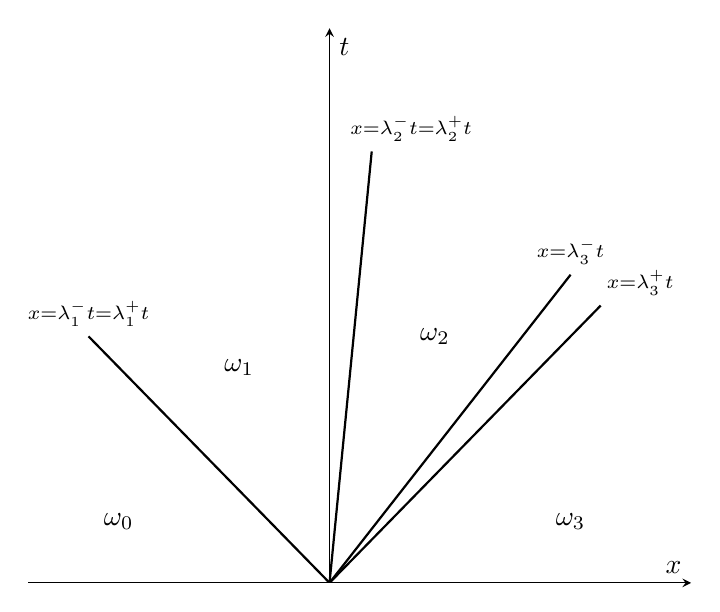
\begin{tikzpicture}
	\begin{axis} [axis lines = middle, ymin=0, ymax=9, xmin=-5, xmax=6, xlabel={$x$}, ylabel={$t$},  width=10cm, xmajorticks=false, ymajorticks=false]
            \addplot[domain=-4:0,samples=200, smooth, thick]{-1*x} 
            node[above,pos=0]{$\scriptstyle{x=\lambda_{1}^{-}t=\lambda_{1}^{+}t}$}
            node[] at (axis cs: -3.5,1) {$\omega_{0}$};
            \addplot[domain=0:0.7,samples=200, smooth, thick]{10*x}
            node[above]{$\hspace{1cm}\scriptstyle{x=\lambda_{2}^{-}t=\lambda_{2}^{+}t}$}
            node[] at (axis cs: -1.5,3.5) {$\omega_{1}$};
            \addplot[domain=0:4,samples=200, smooth, thick]{1.25*x}
            node[above]
            {$\scriptstyle{x=\lambda_{3}^{-}t}$}
            node[] at (axis cs: 1.75,4) {$\omega_{2}$};
            \addplot[domain=0:4.5,samples=200, smooth, thick]{x}
            node[above]
            {$\hspace{1cm}\scriptstyle{x=\lambda_{3}^{+}t}$}
            node[] at (axis cs: 4,1) {$\omega_{3}$};
	\end{axis}
    \label{plot:2.5}
\end{tikzpicture}
\caption{}
\end{center}
\end{figure}

Consideriamo un sistema $3\times 3$, assumendo che il primo e il terzo campo caratteristico sono genuinamente non lineari, mentre il secondo è linearmente degenere. Il grafico mostra la struttura della soluzione $u=u(t,x)$ nel caso in cui $\sigma_{1}<0, \sigma_{2}\neq 0$ e $\sigma_{3}>0$. In questo caso la soluzione contiene due shock, uno viaggiante con velocità $\lambda_{1}^{\pm}=\lambda_{1}(\omega_{0},\omega_{1})$ e uno avente velocità $\lambda_{2}^{\pm}=\lambda_{2}(\omega_{1})=\lambda_{2}(\omega_{2})$. Inoltre nel settore dove $x/t\in [\lambda_{3}^{-},\lambda_{3}^{+}]=[\lambda_{3}(\omega_{2}),\lambda_{3}(\omega_{3})]$, la soluzione contiene una rarefazione centrata.\\
Dimostriamo ora che esiste una simile soluzione del problema di Riemann.
\begin{teorema}
    Supponiamo che il sistema \eqref{eq:2.20} sia strettamente iperbolico con coefficienti lisci, definiti in un insieme aperto $\Omega\subseteq\mathbb{R}^{n}$ e che per ogni $i\in\{1,\ldots,n\}$, l'$i$-esimo campo caratteristico sia genuinamente non lineare oppure linearmente degenere.\\
    Allora per ogni insieme compatto $K\subset\Omega$, esiste un $\delta >0$ tale che il problema di Riemann \eqref{eq:2.20}-\eqref{eq:2.21} ha un'unica soluzione debole della forma \eqref{eq:2.74}, per $u^{-}\in K, \|u^{+}-u^{-}\|\leq\delta$.
\end{teorema}
\begin{proof}
    Sia $u^{-}\in\Omega$ fissato. La mappa $\Lambda$ definita in \eqref{eq:2.69} è derivabile con continuità due volte con derivata seconda lipschitziana e soddisfa
    \begin{equation}\label{eq:2.75}
        \left.\frac{\partial\Lambda}{\partial\sigma_{i}}\right|_{\sigma_{1}=\ldots=\sigma_{n}=0} = r_{i}(u^{-}).
    \end{equation}
    Siccome gli $n$ autovettori $r_{1}(u^{-}),\ldots,r_{n}(u^{-})$ sono linearmente indipendenti, ho che
    \begin{equation*}
            \det\left[ D_{\sigma}\Lambda(0,\ldots,0)(u^{-})\right]=\det\left[ r_{i}(u),\ldots,r_{n}(u) \right]\neq 0,
        \end{equation*}
    allora per il teorema della funzione inversa la mappa
    \begin{equation*}
        (\sigma_{1},\ldots,\sigma_{n})\mapsto\Lambda(\sigma_{1},\ldots,\sigma_{n})(u^{-})
    \end{equation*}
    è un omeomorfismo $C^{2}$ da un intorno di $0\in\mathbb{R}^{n}$ in un intorno di $u^{-}$. Dunque esiste un $\delta >0$ tale che, per ogni $u^{-}\in K$, se $\|u^{+}-u^{-}\|\leq\delta$ allora $u^{+}=\Lambda(\sigma_{1},\ldots,\sigma_{n})(u^{-})$ per qualche $\sigma_{1},\ldots,\sigma_{n}$. In questo caso la funzione $u$ definita in \eqref{eq:2.74} fornisce una soluzione debole per il problema di Riemann.
\end{proof}